\documentclass[danish]{article}

\usepackage{fullpage}
\usepackage[latin1]{inputenc}
\usepackage[danish]{babel}
\usepackage{listings}
%\usepackage{color}
\usepackage{xcolor}
\usepackage{amssymb}
\usepackage{amsmath}
\usepackage{fancyhdr}
\usepackage{lastpage}
%\usepackage{textcomp}
\usepackage{hyperref}
\usepackage{parskip}
\usepackage{graphicx}
\usepackage{epstopdf}

% setup c sharp syntax highlight
\lstdefinestyle{sharpc}{
  language=[Sharp]C, 
  frame=lr, 
  rulecolor=\color{black},
  basicstyle=\footnotesize\ttfamily,
  keywordstyle=\bfseries\color{green!40!black},
  commentstyle=\itshape\color{purple!40!black},
  identifierstyle=\color{blue},
  stringstyle=\color{orange}}

\lstset{
  style=sharpc, 
  numbers=left,
  escapeinside={\<*}{*>},     
  breakatwhitespace=true  }

% code formatting helper
\newcommand{\code}[1]{\texttt{#1}}

% no paragraph indention
\setlength{\parindent}{0pt}

% setup page style
\pagestyle{fancy}
\fancyhf{}
\setlength{\headheight}{15pt}
\setlength{\headsep}{25pt}
\lfoot{Side \thepage{} af \pageref{LastPage}}
\rfoot{30/04-2013}
\lhead{02105 - Algo 1}
\chead{Skattejagt}
\rhead{Simon Altschuler (s123563)}



\begin{document}
\section{Introduktion}
I hver af foelgende opgaver og implementationer har jeg brugt C\#. Jeg har parset input dataen til variablen \code{string mapString}, \emph{uden} den foerste linie (n-linien). \code{mapString} antages at eksistere i kode eksemplerne. I opgaverne B, C og D er denne streng yderligere parset til variablen \code{List<char[]> map}, altsaa en to-dimensionel liste som repraesenterer kortet, og hvor et koordinat tilgaas ved \code{map[y][x]}, da de indre lister i \code{map} repraesenterer raekker i stedet for kolonner, grundet simplere parsing.

Parsingen af data'en er ikke medregnet i algoritme analyserne.

\section{Antal skatte}
\subsection{Beskrivelse}
Jeg itererer hver karakter i \code{mapString}, og for hver af dem som er lig karakteren ``\$'' laegger jeg 1 til variablen \code{int amount}, som indeholder svaret naar loekken er koert.

\subsection{Implementation og analyse}
Bemaerk at \code{mapString} her er en streng \emph{uden} linieskift karaktere, altsaa en $n^2$ lang streng.
\begin{lstlisting}
var amount = 0;                        // <*$c$*>
foreach (var ch in mapString)          // <*$n$*>
    if (ch == '<*\$*>')                     // <*$n^2$*>
       amount++;                       // <*$n^2$*>

Console.WriteLine(amount);             // <*$c$*>
\end{lstlisting}

Hver linies antal eksekveringer er noteret som kommentare. Samlet har jeg foelgende udtryk for tidskompleksiteten som funktion af kortets stoerrelse $n$:
\[ 2n^2 + n + 2c \]
Naar jeg smider konstanten vaek ender jeg op med $n^2$ som den hoejst betydende faktor og dermed er worst-case koeretiden $\theta{}(n^2)$. Det giver intuitivt mening, da hvert felt i kortet tjekkes praecis een gang, og kortets antal felter er $n^2$, hvilket ogsaa viser at algoritmen er korrekt, da alle mulige skatte itereres. 

\section{Tilg�ngelige skatte}
\subsection{Beskrivelse}
Til opgaven bruger jeg BFS\footnote{Breadth First Search} algoritmen. Kortet opfattes som vaerende en graf i sig selv, hvor hvert koordinat er en knude og hver nabo til en knude som ikke er vaeg (\code{\#}), indikerer en kant til foerende naboen. 

Jeg bruger en koe (\code{Queue<Tile> frontier} i C\#) som datastruktur for de felter/koordinater (\code{Tile}s), der skal undersoeges, og jeg markerer et felt udforsket ved at aendre det til en vaeg i kortet (\code{map}). Paa den maade vil et felt aldrig blive tilfoejet til \code{frontier} mere end een gang.

Jeg initialiserer en variabel \code{found} (linie \ref{code:b_found}) til at gemme antallet af fundne skatte.

Jeg laegger indgangsfeltet i koeen, og saetter en \code{while} loekke igang (linie \ref{code:b_while}), som koerer indtil \code{frontier} er tom. Hver iteration i loekken ``Dequeue''er naeste knude (\code{Tile}) i koeen (foerste gang dermed indgangsfeltet) og laegger dens naboer ind i \code{frontier}, hvis det er et gyldigt felt (dvs. ikke-vaeg, og inden for kortets rammer). For hver af dets naboer som er en skat, laegges 1 til antal fundne skatte (linie \ref{code:b_found_up}).

Dermed bliver hver knude tjekket een gang, men kun de knuder som kan naas fra indgangsfeltet, da knuder som er spaerret inde af vaegge aldrig kan blive tilfoejet til frontier. Det kan de ikke fordi de ikke har nogle kanter som foerer ind til de tilgaengelige knuder/felter.

Figur \ref{fig:map_b} viser hvordan algoritmen gaar fra felt til felt, visualiseret ved en pil. Det bemaerkes at der kun er een pil som pejer paa hvert felt ($deg^-(v) = 1$), men der kan vaere fra $0-3$ ud ($deg^+(v) \in \{0,1,2,3\}$). Dermed er grafen over de tilgaengelige skatte et (orienteret) trae som er et sammenhaengskomponent i den samlede graf over kortet.

\begin{figure}[!htb]
  \centering
  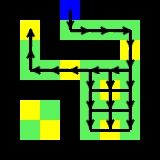
\includegraphics[width=30mm]{map_b.jpg}
  \label{fig:map_b}
  \caption{Sample02 fra E-Judge; blaa: indgang, groen: gulv, gul: skat, sort: vaeg}
\end{figure}

\subsection{Implementation}
\begin{lstlisting}
var entry = new Tile();
// find indgangen, antag at der er praecis en (tager foerste)
for (var y = 0; y < n; ++y)
    for (int x = 0; x < n; ++x)
        if (map[y][x] == 'I') 
        {
          entry = new Tile(x, y);
          break;
        }

// initialiser en koe over felter som skal undersoeges
var frontier = new Queue<Tile>();
// tilfoej indgangen som foerste felt der skal undersoeges
frontier.Enqueue(entry);
// variabel som bruges til at taelle tilgaengelige skatte
<*\label{code:b_found}*>var found = 0;
<*\label{code:b_while}*>while (frontier.Count > 0)
{
    // tag foerste element ud af koeen
    var curr = frontier.Dequeue();
    // saet feltet som vaerende vaeg for ikke at undersoege det igen
    map[curr.Y][curr.X] = '#';
    
    // undersoeg om felter oven, under, til hoejre 
    // og til venstre er gyldige at gaa videre paa
    ProcessTile(n, curr.X-1, curr.Y, ref found, frontier, map);
    ProcessTile(n, curr.X+1, curr.Y, ref found, frontier, map);
    ProcessTile(n, curr.X, curr.Y+1, ref found, frontier, map);
    ProcessTile(n, curr.X, curr.Y-1, ref found, frontier, map);	
}

Console.WriteLine(found);

// funktionen ProcessTile som bruges ovenfor
void ProcessTile(int n, int px, int py, ref int found, 
                 Queue<Tile> frontier, List<char[]> map)
{
    // tjek om koordinatet er inden for kortets rammer
    // og at den i saa fald er gyldig at gaa videre paa (ikke er vaeg)
    if (!(px < 0 || py < 0 || px > (n-1) || py > (n-1)) && map[py][px] != '#')
    {
	var p = new Tile(px, py);
	// tael en op hvis feltet er en skat
	if (map[py][px] == '<*\$*>') 
	    <*\label{code:b_found_up}*>found++;
	// tilfoej feltet til koeen over felter der skal gaas videre paa
	frontier.Enqueue(p);
	// saet feltet som vaerende ugyldig at tilfoeje til listen 
	// over utjekkede felter (der er netop blevet gjort og maa ikke goeres igen)
	map[py][px] = '#';
    }
}
\end{lstlisting}

\subsection{Analyse}
For simplicitet har jeg analyseret koden i grupper af linier:
\begin{description}
  \item[Linie 1] $c$
  \item[Linie 3] $n$
  \item[Linie 4-5] $n^2$
  \item[Linie 12-16] $3c$
  \item[Linie 17-29] $n^2$, da \emph{alle} tiles i worst-case tjekkes
  \item[Linie 40] $4n^2$, da den for hvert felt der tjekkes kaldes 4 gange
  \item[Linie 42-50] $n^2$, da praemissen i linie 40 maksimalt vil opfyldes $n^2$ gange grundet ``vaeg-tjekket''
\end{description}

Dermed er den samlede worst-case koeretid 
\[ 7n^2 + n + 4c \]
Og derfor i $\theta$ notation: $\theta{}(n^2)$. Jvf. slides brugt i undervisningern er koeretiden af BFS

BFS loeber i worst-case alle kanter og knuder igennem  har koeretiden $\theta{}(v+e)$, hvor $v$: knuder, $e$: kanter
\section{Den bedste indgang}
\subsection{Beskrivelse}
BFS hvor indgange fjernes hvis den finder en ny indgang foer en skat. Itererer alle resterende indgange.
\end{document}